\subsection{Análise semanal}
O ponto principal para a decisão a respeito da utilização da agregação semanal na gestão da central de atendimento é a existência de diferenças entre as amostras semanais, as quais justificariam a adoção desse nível de agregação mais detalhado.\\
O teste não paramétrico de Kolgomorov Smirnov foi novamente utilizado para realização do teste de hipótese. Para que não houvesse uma matriz desnecessariamente grande, contendo testes dois a dois para cada uma das 52 semanas de um ano (matriz 52x52), foram representadas apenas as primeiras oito semanas do ano e as últimas oito semanas do ano.

\begin{figure}[H]
    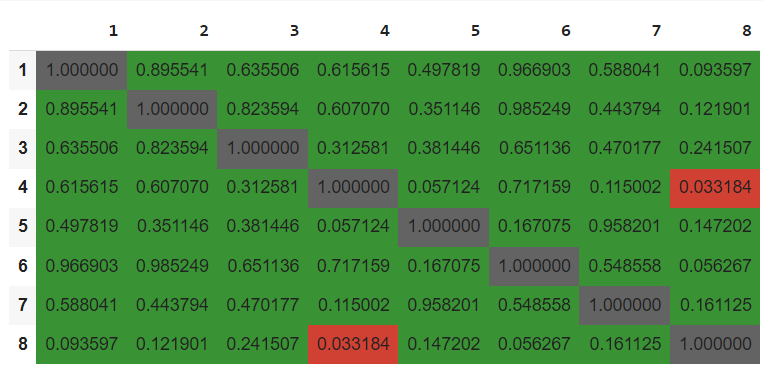
\includegraphics{analise-de-dados/semanal/janas.png}
    \caption{Kolgomorov Smirnov - teste para intervalos de chegada nas oito primeiras semanas de 2021}
    \label{fig: jan_as_img}
\end{figure}

\begin{figure}[H]
    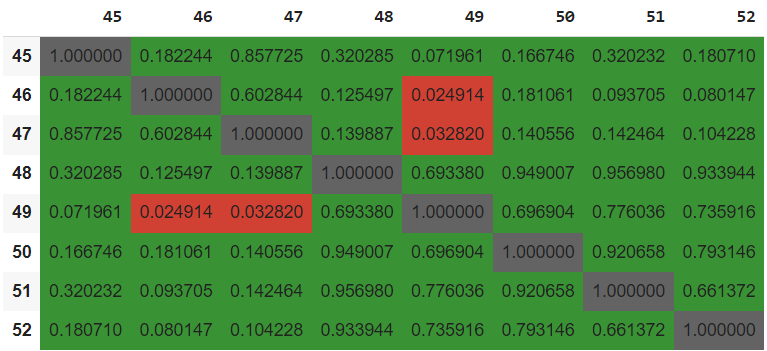
\includegraphics{analise-de-dados/semanal/dezas.png}
    \caption{Kolgomorov Smirnov - teste para intervalos de chegada nas oito últimas semanas de 2021}
    \label{fig: dez_as_img}
\end{figure}

A Figura \ref*{fig: jan_as_img} mostra o teste de Kolmogorov-Smirnov para os tempos de intervalo entre chegadas nas primeiras oito semanas do ano. A Figura \ref*{fig: dez_as_img} apresenta o teste de hipóteses para os tempos de intervalo entre chegadas nas últimas oito semanas do ano.\\
Foi possível observar que no horizonte de planejamento semanal, semanas subsequentes tendem a ter intervalos de chegada que seguem a mesma distribuição de probabilidade e, portanto, o planejamento semanal não é interessante para esse problema, visto que não é possível perceber as diferenças de demanda nesse nível de análise.